
\section*{Trusted Path}

SGX-style enclaves provide secure \emph{computation}, as their execution is isolated from other software on the same platform. However, they do not easily lend themselves to secure \emph{user interaction}. The main reason for this is that, in an architecture like SGX, enclaves communicate with I/O devices through the untrusted OS. When an enclave needs to receive user input, it is the responsibility of the OS to pass data from an input device like keyboard or mouse to the enclave. When an enclave needs to send user output, it is the responsibility of the OS to forward output data received from the enclave to a user output device like the screen. Such TEE design means that a compromised OS can easily modify any user input and output and read any secrets that are communicated between the user and the enclave. 

User input manipulation can have severe consequences in several application scenarios. For example, if a malicious OS modifies user input that is provided to a financial enclave, the enclave could be tricked to perform unauthorized payments. If enclaves are used to control safety-critical system such as a medical devices or industrial systems, user input modifications may cause serious safety risks. Also any enclave that needs to be configured with a password or similar user authentication credential is difficult to implement securely.

Such lack of secure user interaction capabilities means that SGX enclaves do not support \emph{trusted path}~\cite{x86} --- a secure channel from the human user to the trusted application. 

%Depending on the application scenario, two different types of trusted paths may be desirable. The first, and more common, definition of trusted path is a secure communication channel between the human user and a \emph{local} trusted application like an enclave. The second, and perhaps less common, definition of trusted path is one that realizes a secure communication channel between the user and the \emph{remote} server without using any trusted local application in between. 


\subsubsection*{Design Principles}

Several projects have explored the idea of complementing commodity computing platform with additional trusted hardware that would enable a trusted path. While proposing extra hardware may be easy, the more difficult question is: what should the added hardware do to realize a trusted path? To answer this question, we look at noteworthy previous approaches. By examining the main limitations of previous solutions, we can identify design principles for more secure trusted path.
	
The first approach that we examine is \textbf{transaction confirmation}~\cite{filyanov2011uni}. In such a solution, the user first completes the user interaction, such as payment, by interacting with the user interface of the untrusted platform. Once this is done, the user is expected to confirm his input, like a payment value and account number, from the display of a separate hardware token, in order to detect any possible input value modifications.

This approach has two main problems. The first problem is that the user now has to interact with two separate user interfaces which reduces usability. The second, and more severe, problem is that such extra confirmation step is vulnerable to \emph{user habituation}, i.e, the possibility that user starts, after few successful transactions, confirming new payments without actually verifying their correctness. These observations lead us to the first design principle.  

\begin{tcolorbox}
\textbf{Principle 1:} Out-of-context security confirmations have high cognitive load and risk of user habituation. Thus, user interaction should be protected in-context of the normal user interface.
\end{tcolorbox}

The next known approach that we examine is \textbf{input trace signing}~\cite{IntegriKey}. Here, the main idea is to use a simple hardware device that sits in-between a user input device, such as keyboard, and the untrusted computing platform. The device intercepts and signs every keypress, or similar user input event, and sends a signed trace to the trusted application. This approach is also known as ``bump-in-the-wire''~\cite{McCPerRei2006}. 

This approach meets our first principle, because the user does not have to perform additional security checks outside the main UI. However, such solutions are vulnerable to attacks, where the adversary manipulates user's input by showing false information on the output channel. One example is \emph{fake-typo} attack. Assume that the user types in value ``10'', but the adversary shows ``1'' on the screen. The user is likely to think that he mistyped and press ``0'' again. As a result, signed trace of ``100'' will be sent to the trusted application. This simple attack leads us to our next design principle.

\begin{tcolorbox}
\textbf{Principle 2:} User input and output integrity cannot be considered in isolation. Both must be protected simultaneously.
\end{tcolorbox}

The third and last approach that we examine is \textbf{secure overlays}. Fidelius~\cite{Fidelius} is an example of this approach. The solution is based on two separate devices. One device intercepts keyboard presses and signs them for the trusted application. Another device intercepts the HDMI output signal and modifies it with secure overlays of of security critical UIs such as payment web forms. 

Fidelius addresses the above mentioned problems, but is still vulnerable different type of user input manipulation that we call ``early-submission attack''. This attack is rooted in the fact that a system like Fidelius only protects the integrity of the keyboard input, but not other user input peripherals like mouse. Assume again, that the intention of the user is to type value ``10''. Once user has typed ``1'', the untrusted computing platform generates a fake mouse event that completes and submits the web form. Given this attack, we can state our last design principle.

\begin{tcolorbox}
\textbf{Principle 3:} All user input modalities must to be protected simultaneously.
\end{tcolorbox}


\subsubsection*{\protection system}

The model is depicted in Figure~\ref{fig:approachOverview} which shows the untrusted host, the remote server, and the user IO devices. We only assume that the monitor, keyboard, mouse (in a word all the IO devices that we need to protect from the malicious host) and the \protection are trusted. The \protection works as a mediator between all the IO devices and the host. Note that the \protection has no network capability to communicate with the server directly, rather it relies on the host and uses it as an untrusted transport. We also assume that the \protection comes with preloaded certificates and keys that allow the \protection to verify the signatures signed by the server and sign data such as the user input.

\begin{figure}[t]
	\centering
	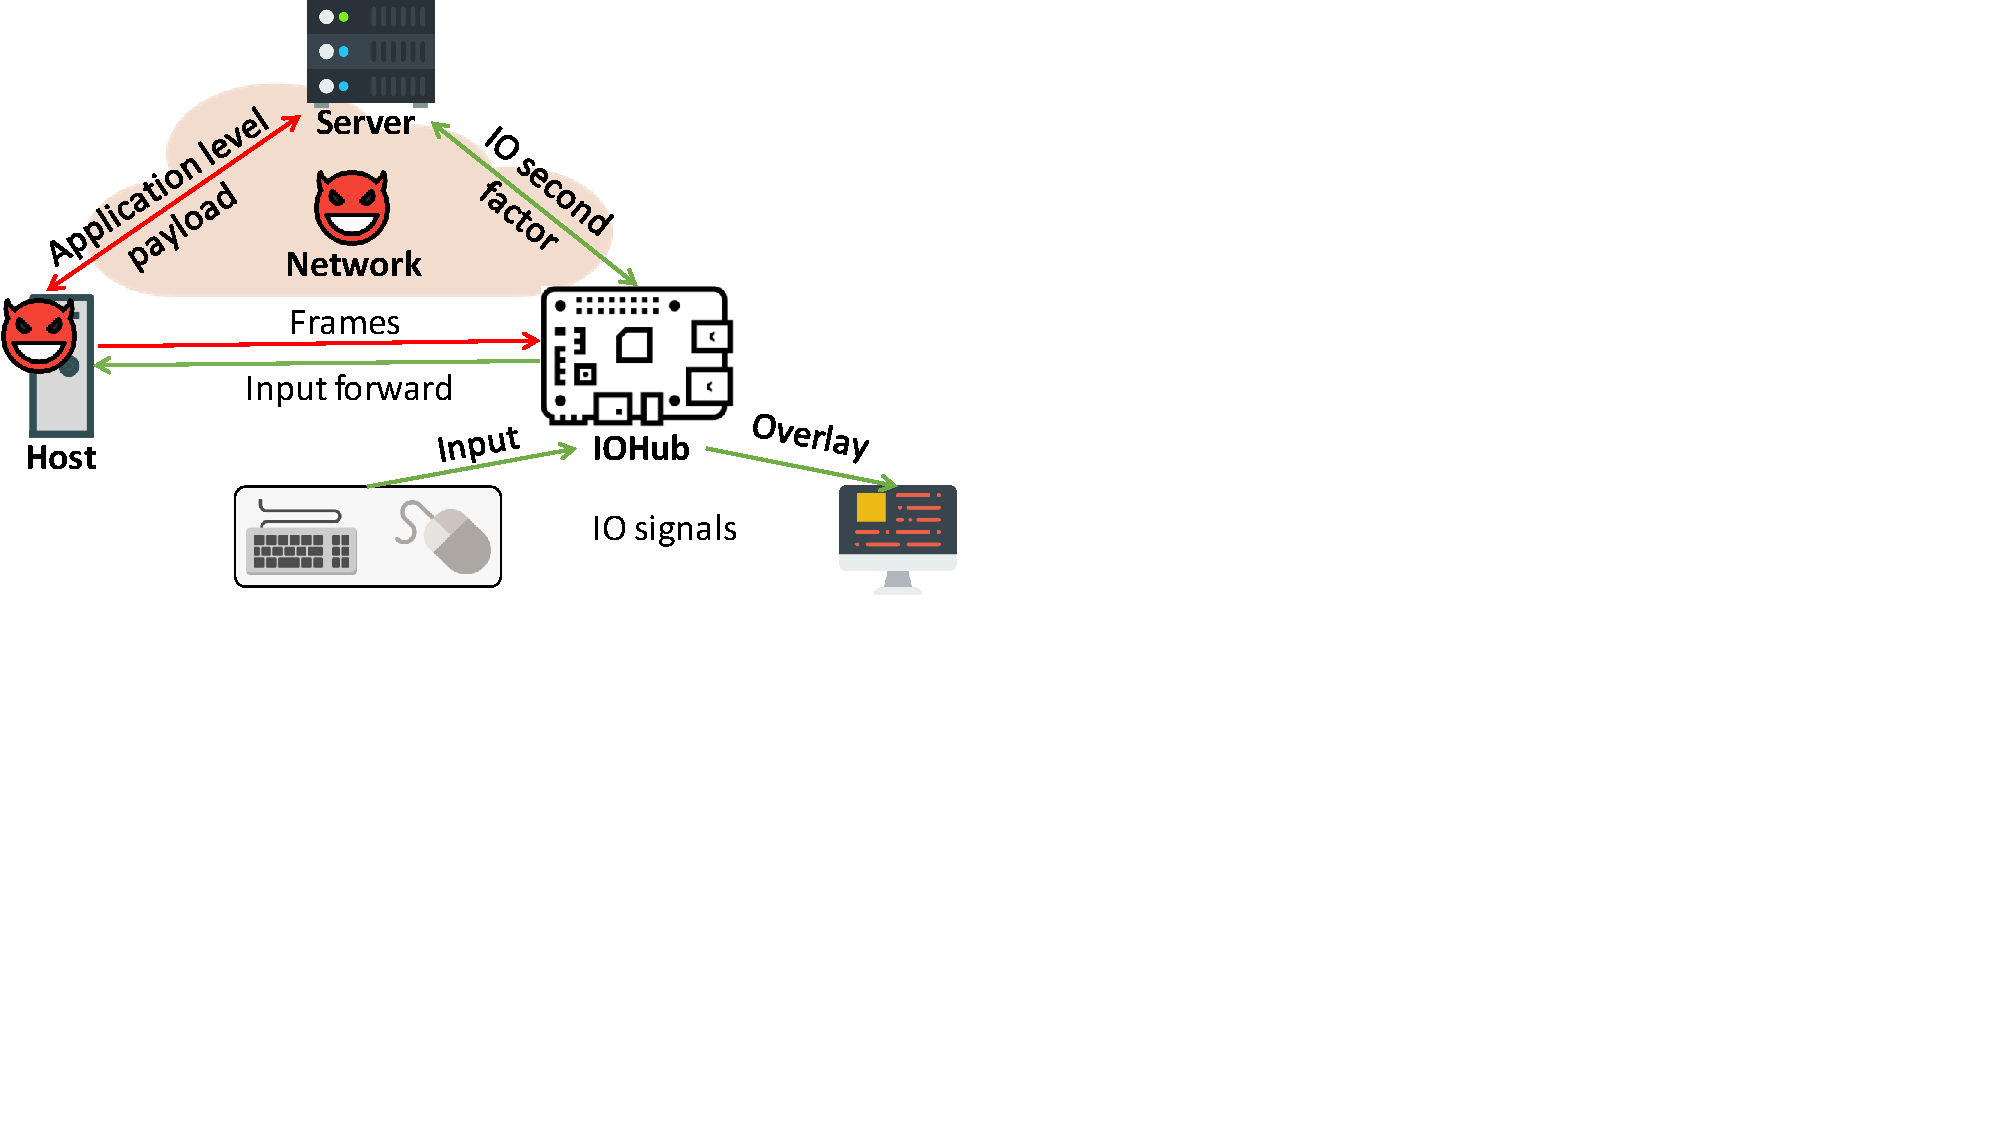
\includegraphics[trim={0 8.5cm 17cm 0}, clip, width=0.9\linewidth]{approachOverview.pdf}
	\caption{\protection architecture.}
	\label{fig:approachOverview}
\end{figure}

\begin{figure}[t]
	\centering
	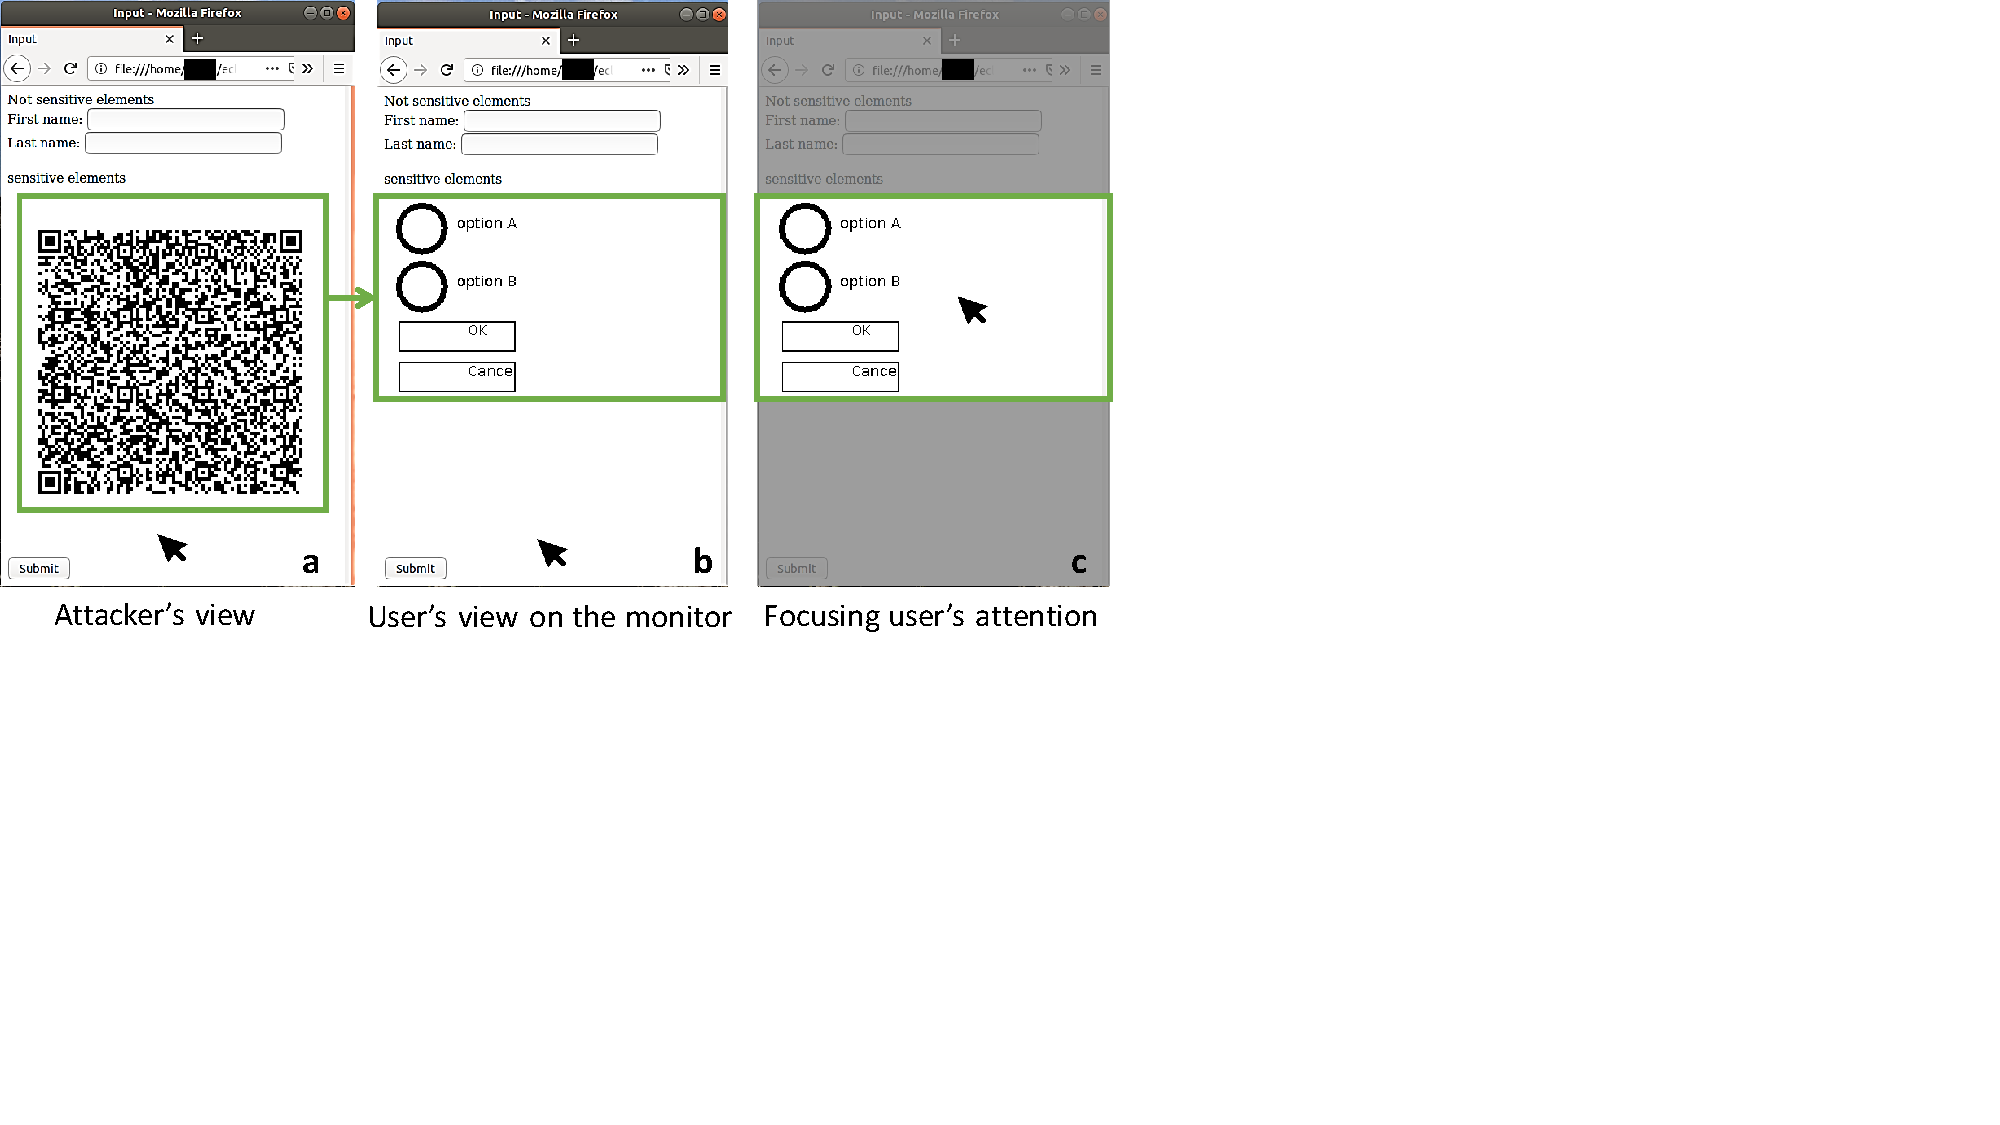
\includegraphics[trim={0 8cm 15cm 0}, clip, width=\linewidth]{overlayScreenShot_new.pdf}
	\caption{\protection user interface.}
	\label{fig:screenshot_1}
\end{figure}

There are many possible ways to deploy \protection. One way is to assume that the \protection manufacturer issues a certificate for each of the deployed \protection{}s . The \protection maintains a whitelist for the remote servers along with their public certificates. This allows the \protection to verify messages signed by those remote servers. Another assumption could be that the \protection is issued by a service provider who also runs the remote server. 

\protection is build upon the security requirements and functional properties that are described in Section~\ref{goals}. 
\protection is active only when the user visits sensitive web applications that require \name security.
Initially, the remote server signs and delivers the sensitive UI elements to the host in a format that is understandable by \protection. Next, the host transfers the sensitive UI to \protection, and the \protection verifies the signature to prevent manipulations by the host. As seen in a running example depicted in Figure~\ref{fig:screenshot_1}, the \protection then renders the UI with sensitive elements into an overlay on top of the HDMI frame received from the host. Note that the host cannot access or modify the overlay generated by the \protection. Also, the overlay covers only a part of the screen, allowing the other feature-rich content on the webpage to run unmodified. Therefore, this ensures that sensitive UI elements are presented to the user as expected by the remote server -- \emph{output integrity}. For the overlay, we use QR-codes to transfer data from the host to the device because we avoid using extra software/hardware for a separate channel, and it is easy to visualize.

When the user interacts (types or moves the pointer) with the overlay, \protection does not forward any event from the keyboard or the mouse to the host. The interaction is maintained solely by \protection, which renders on-screen user inputs and therefore offers a user experience that is identical to a typical one as if the \protection is not present. The user click on the \emph{submit} button triggers the submission procedure, which consists of the \protection signing the user inputs and sending to the server. Note that the text fields of the form and the \emph{submit} button are inside the overlay which is inaccessible by the host, hence the attacker cannot execute the early form submission or clickjacking attacks. Finally, the server verifies the signature of \protection to guarantee that the host has not altered the data. Therefore, the \protection ensures \emph{input integrity} for all \emph{modalities} of input.

For integrity guarantees, \name uses well-known user attention focusing mechanisms such as lightbox that aid the user to distinguish the \protection overlay on the screen from the rest. Thus, the untrusted host cannot trick the user into following malicious instructions when the user interacts with sensitive UI elements. Also, the host cannot observe sensitive data on the overlay because it does not have access to it. In the case where confidentiality is required, the user manually triggers SAS, such as the lightbox by pressing specific keys.


\subsubsection*{Prototype and Deployment}

\begin{figure}[t]
	\centering
	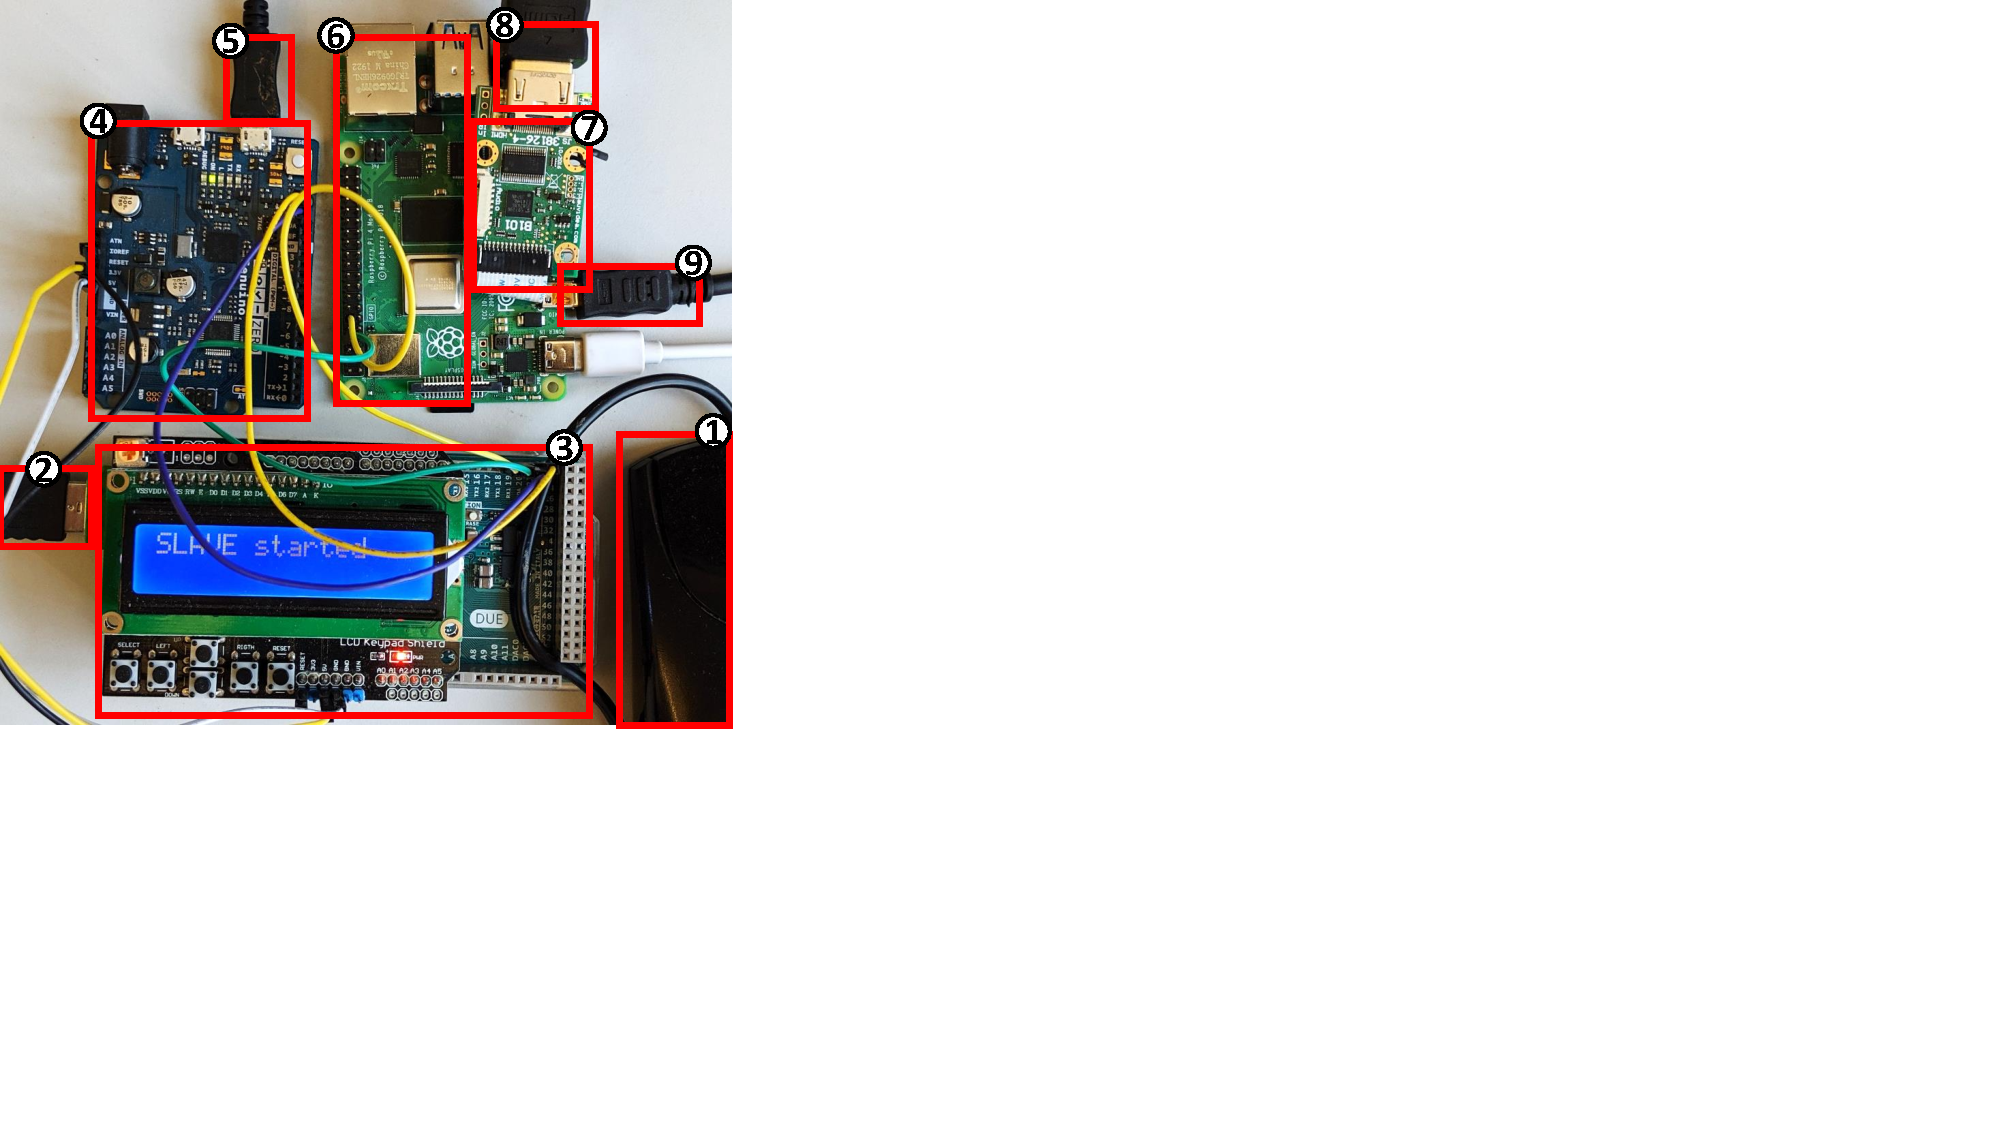
\includegraphics[trim={0 6.6cm 21.5cm 0}, clip, scale=0.5]{setUp_1.pdf}
	\caption{\protection prototype.}
\label{fig:prototypeArch}   
\end{figure}

Figure~\ref{fig:prototypeArch} shows our \protection prototype.
The delay in forwarding keystrokes is $170\ \mu s$ and for frames is $21.76\ ms$. This allows the \protection to achieve the maximum display frame rate of $47.69$ per second (e.g., most of the movies are shot and shown in  ~24-30 fps).

Deployment...





